\documentclass[tikz,border=10pt]{standalone}
\usepackage{amssymb} % for \subset
\usepackage{pgf,tikz,pgfplots,tkz-euclide}
\usepackage{tikz-3dplot}
\pgfplotsset{compat=1.15}
\usepackage{mathrsfs}
\usepackage{amsmath}
\allowdisplaybreaks[4]
\usetikzlibrary{arrows,arrows.meta,angles,quotes,automata,math}
\usetikzlibrary{calc,fadings,decorations.pathreplacing}
\usetikzlibrary{shadings,intersections}
\usetikzlibrary{3d}
\usetikzlibrary{hobby}
%\usepackage{amsthm}
\usepackage{wrapfig}
\usepackage{gensymb}
\usepackage{subfigure} 
\usepackage{physics}
\usepackage{diagbox}

\begin{document}

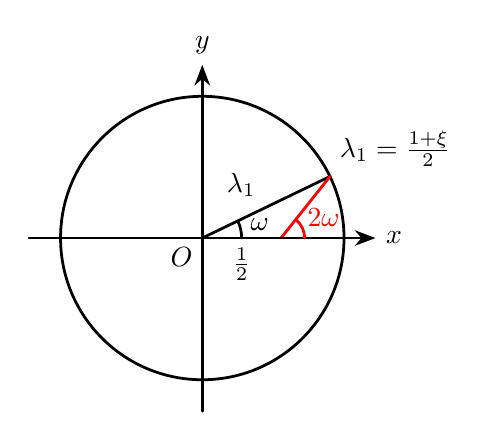
\begin{tikzpicture}[cap=round,scale=2]
\coordinate[] (A) at (0.811, 0.391);
\coordinate[] (M) at (0.5,0);
\coordinate (X) at (1,0);
\coordinate[label=below left:$O$] (O) at (0,0);
\draw [line width=1pt] (O) circle (0.9cm);
\draw [line width=1pt] (O) to [edge label=$\lambda_1$] (A);
\draw [line width=1pt,red] (M) -- (A);
\draw[-Stealth,line width=1pt] (-1.1,0) -- (1.1,0) node[right] {$x$};
\draw[-Stealth,line width=1pt] (0,-1.1) -- (0,1.1) node[above] {$y$};
\draw[anchor=north] (0.25,0) node {$\frac{1}{2}$};
\draw[anchor=south west] (A) node {$\lambda_1 = \frac{1+\xi}{2}$};
\draw pic["$\omega$",draw,line width=1pt, angle eccentricity=1.5, angle radius=0.5cm] {angle=X--O--A};
\draw pic["$2\omega$",draw,line width=1pt,red,angle eccentricity=2.0, angle radius=0.3cm] {angle=X--M--A};
\end{tikzpicture}

\end{document}